\documentclass[12pt,letterpaper]{article}
\usepackage{setspace}
\usepackage{scalerel}
\usepackage{amsmath, amsthm, amsfonts, amssymb}
\DeclareMathOperator*{\rint}{\ThisStyle{\rotatebox{15}{$\SavedStyle\!\int\!$}}}
\usepackage{indentfirst}
\usepackage[colorlinks=true,linkcolor=black,urlcolor=blue,citecolor=black]{hyperref}
\usepackage{bm}
\usepackage{caption}
\usepackage{subcaption}
\usepackage{graphicx}
\usepackage{epstopdf}
\usepackage{mathpazo}
\usepackage{float}
\usepackage{pgfplots}
\usepackage[affil-it]{authblk}
\pgfplotsset{compat=1.16}
\usepackage{dcolumn}
\usepackage{booktabs}
\usepackage{afterpage}
\usepackage[default]{lato}
\usepackage[makeroom]{cancel}
\usepackage{listings}
\usepackage{lscape}
\usepackage[left=2.5cm,right=2.5cm,top=1.5cm,bottom=1.5cm]{geometry}
\usepackage{etoolbox}% http://ctan.org/pkg/etoolbox
\BeforeBeginEnvironment{tabular}{\footnotesize}% Adjust tabular font size to \small

%% BibTeX settings
\usepackage[square,sort,comma,numbers]{natbib}
\bibliographystyle{apalike}
\bibpunct{(}{)}{,}{a}{,}{,}



% Defines columns for tables
\usepackage{array}
\newcolumntype{L}[1]{>{\raggedright\let\newline\\\arraybackslash\hspace{0pt}}m{#1}}
\newcolumntype{C}[1]{>{\centering\let\newline\\\arraybackslash\hspace{0pt}}m{#1}}
\newcolumntype{R}[1]{>{\raggedleft\let\newline\\\arraybackslash\hspace{0pt}}m{#1}}


\definecolor{blue}{RGB}{0,114,178}
\definecolor{red}{RGB}{213,94,0}
\definecolor{yellow}{RGB}{240,228,66}
\definecolor{green}{RGB}{0,158,115}
\definecolor{dkgreen}{rgb}{0,0.6,0}
\definecolor{gray}{rgb}{0.5,0.5,0.5}
\definecolor{mauve}{rgb}{0.58,0,0.82}

\hypersetup{
	colorlinks=false,
	linkbordercolor = {white},
	linkcolor = {blue}
}



\title{The Impacts of Genomic Selection on the American Livestock Genetics Market} 
\author[1]{Victor Funes-Leal}
\author[2]{Jared Hutchins}
\affil[1]{Department of Agricultural and Consumer Economics\\ University of Illinois}
\affil[2]{Department of Agricultural and Consumer Economics\\ University of Illinois}


\date{} %date not required

\begin{document}
\maketitle

\section{Introduction}

\begin{abstract}
    \noindent
    We develop a synthetic control group to estimate the long-term impacts of introducing Genomic Selection in the US market for dairy cattle genetics. Using a data set of all bulls' genetics marketed in the US and Canada from 2000 to 2020, we find that genomic selection significantly increased genetic gains for all measured traits, particularly production such as milk, protein, and fat yields, but it is also the source of increased levels of \textbf{inbreeding depression}, a decrease in the performance of animals whose parents have a high degree of relatedness, as a consequence of genetics companies breeding more animals from established lines rather than lesser-known lines with lower trait values but less inbred. We argue that this is a \textbf{network externality} inflicted by genetics companies upon themselves. Solving this externality will require either a mechanism to internalize the harmful effects, such as paying a much higher price for more inbred sires or a collective action mechanism to select which lines will be bred in the next generation.
\end{abstract}

\newpage
\section{Introduction\label{sec:intro}}

Improved genetics via the selection of bulls (sires) and cows (dams) is a crucial driver for productivity improvements in the dairy industry. US milk production has tripled in the last forty years, and over half of this increase is solely due to genetics. The United States is also the world’s largest exporter of bovine genetics, with a share of 46.4\% of the total value of exports in 2019 (Canada is the second largest with a 19.3\% share); every improvement in genetics that takes place in the United States will be quickly transmitted to the rest of the world dairy industry.

\begin{figure}[H]
    \centering
    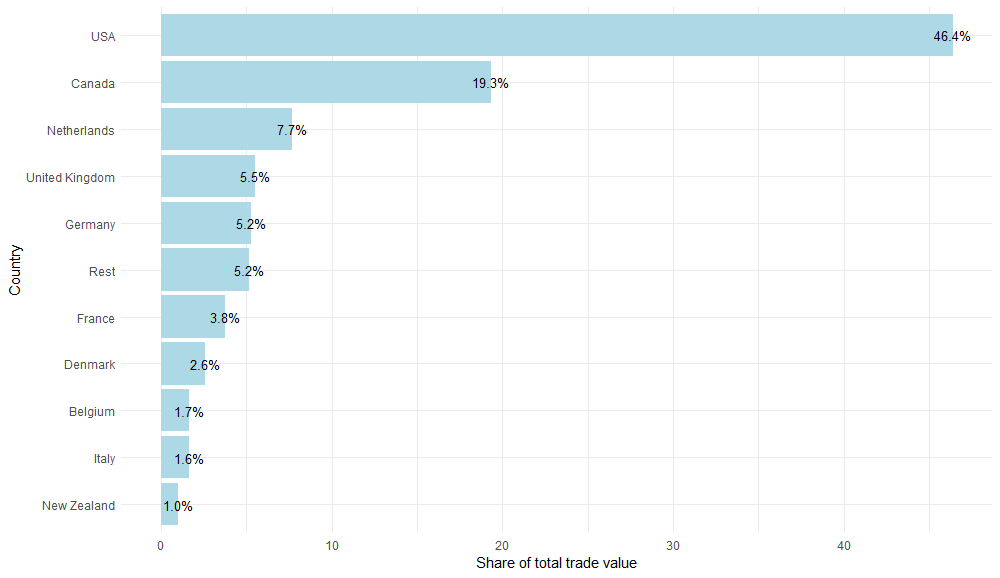
\includegraphics[width=16cm]{figures/semen_exports.png}
    \caption{Share of trade Value of Bovine Semen exports by country (2019)\\ \small \textbf{Source}: UN Comtrade database}
    \label{fig:semen_exp} 
\end{figure}

The demand for cattle genetics is made up of all dairy farmers in the US and abroad who periodically buy bull semen to impregnate their cows for two reasons: a cow needs to be pregnant or weaning her calf to produce milk, and also because they are going to need new cows in the upcoming years; a cow’s productive life is about four years. Dairy farmers rarely keep bulls within their herds because they do not contribute to their profits, so genetics companies provide the semen to impregnate cows. On the other hand, the supply of dairy genetics is constituted by genetics companies that breed bulls to meet the demand for specific traits. To do so, they choose sires and dams with a specific objective. By doing so, they ensure that the next generation of bulls will have a similar or higher level of traits.

Genomic selection uses genetic markers, DNA sequences with a specific location in a chromosome, that cover the entire genome to detect gene combinations whose distribution is significantly different than the expected frequency if they were randomly associated. The most salient consequence of this new method is that it is now possible to test an animal for the presence of markers (which are correlated with specific traits) as soon as the animal is born. What are the consequences of genomic selection? First, it increases the rate of genetic change, that is, the intergenerational variation in the quantities of any genetic trait; this rate of change is a function of how choosy breeders are and how long they must wait for a bull to start fathering his progeny.  

The process of gathering measures of observed traits from an animal’s progeny and using them to estimate their contribution to the traits of his descendants is called evaluation, and it is typically carried out three times a year by the Council on Dairy Cattle Breeding (CDCB)\footnote{\url{https://uscdcb.com/}}. Each trait is a measure of a specific characteristic of the animal’s productivity (milk, fat, protein yield); health (stature, weight, size of udders); or reproduction (calving ability, metritis, gestation length) that a bull will transmit to his offspring, after controlling for factors such as breed, age and, pedigree. In other words, they represent the purely genetic component of the expression of any given characteristic, and that is what a cow fathered by a specific bull will, on average, inherit from him.

In this article, we argue that the introduction of a new method to identify traits in dairy cattle by testing their genome has led to faster gains in production and health traits but has also increased the prevalence of inbreeding depression, a decrease in observed trait values attributable to a higher frequency of recessive genes due to the high relatedness of an animal's parents. We argue that this results from genetics companies supplying more bulls from "prestigious," more inbred pedigrees rather than lesser-known but less inbred alternative pedigrees. Companies do so because there is a demand for high-performance bulls, and their objective is to supply the best possible animals. Unfortunately, they do not consider that the average inbreeding rate across all animals has steadily increased since 2010, and they are now beginning to experience its negative impacts \citep{Cole2019}.

\begin{figure}[H]
    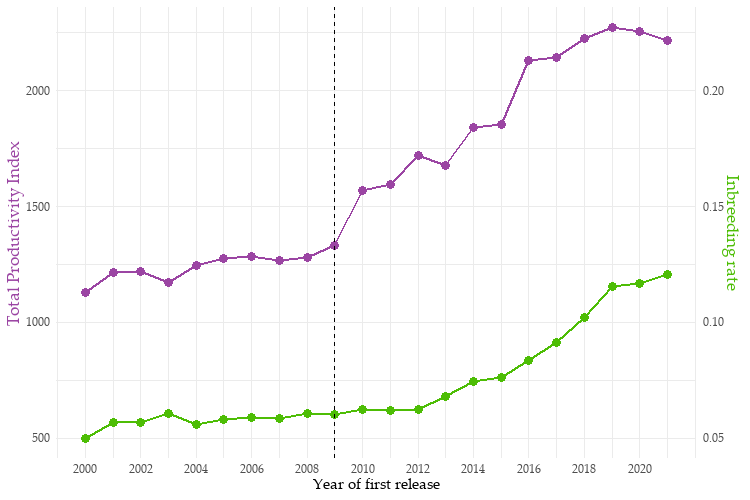
\includegraphics[width=\textwidth]{figures/tpi.png}
    \caption{Average Inbreeding rate and Total Performance Index of Holstein bulls\\ \small \textbf{Source}: NAAB}
    \label{fig:tpi_inb} 
\end{figure}

In economic terms, inbreeding depression can be understood as a negative externality that genetics companies inflict on one another because of genetics companies' increased selection of inbred lines. In this case, the profits of genetics companies are a function of the trait levels of the lines they breed but also depend on the degree of relatedness of such lines to each other. The more genetic companies adopt a line, the higher the likelihood of observing inbreeding depression in the next generation.

This is an example of a \textbf{network externality} \citep{Liebowitz1994}, \citep{Katz1985}, where companies enjoy the benefits (higher trait levels) and suffer the costs (lower fertility levels) from changes in the size of their associated network. In this case, the pedigree (relatedness) is the force that binds all the nodes in the network, where two animals are part of the same network (line) if they descend from the same ancestor. 

The more genetics companies breed the same lines; the more newborn bulls will be related to a specific ancestor and the denser their networks will be. We no longer have a measure of demand strength since the advent of genomic testing, as bull's traits are no longer measured through their daughters. We can, however, approximate it using the number of sons, grandsons, and the rest of his male progeny; a bull with a high level of traits is likely to have a large number of descendants.

Our main finding is that the introduction of genomic selection has led to increased productivity gains. For example, the Total Productivity Index, a weighted average of fourteen genetic traits used to select the best bulls, has increased twofold in 2009-2019, compared to more moderate growth in 2000-2009 (Figure \ref{fig:tpi_inb}.) On the other hand, it has also led to a higher inbreeding among Holstein cattle and, with it, a greater prevalence of inbreeding depression, a negative (indirect) network externality inflicted by genetics companies on themselves by "doubling down" on more popular lines in detriment of less inbred lines. We expect that the cost of inbreeding depression will continue to rise in the following years, but the problem cannot be solved by just breeding fewer inbred bulls; it will also require a mechanism to take into account the inbreeding level of the entire Holstein herd. 


\section{Literature Review}

\section{Conceptual Framework}


\section{Data Description}
\begin{figure}[H]
    \centering
    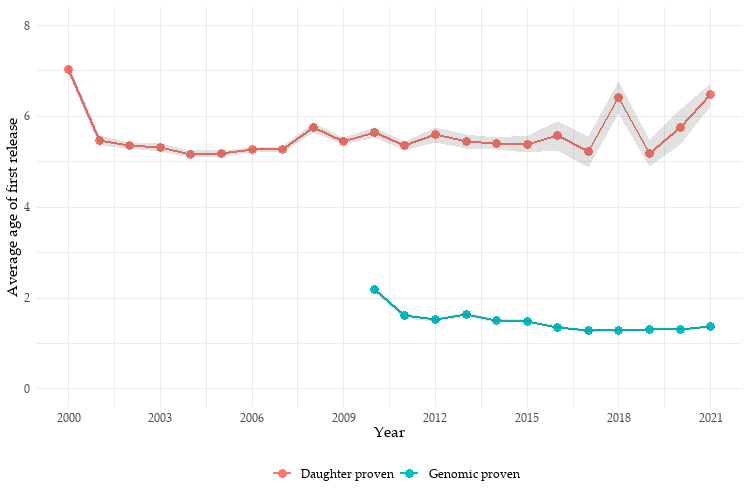
\includegraphics[width=16cm]{figures/generation_interval.png}
    \caption{Average age at first proof for Holstein bulls\\ \small \textbf{Source}: NAAB}
    \label{fig:gen_int} 
\end{figure}

\begin{figure}[H]
    \centering
    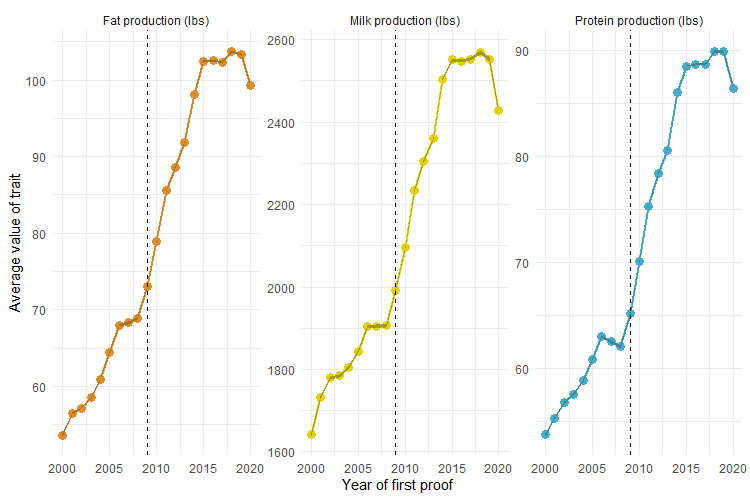
\includegraphics[width=\textwidth]{figures/pta_plots.png}
    \caption{Average value of selected traits\\ \small \textbf{Source}: NAAB}
    \label{fig:pta_plots} 
\end{figure}

\begin{figure}[H]
    \centering
    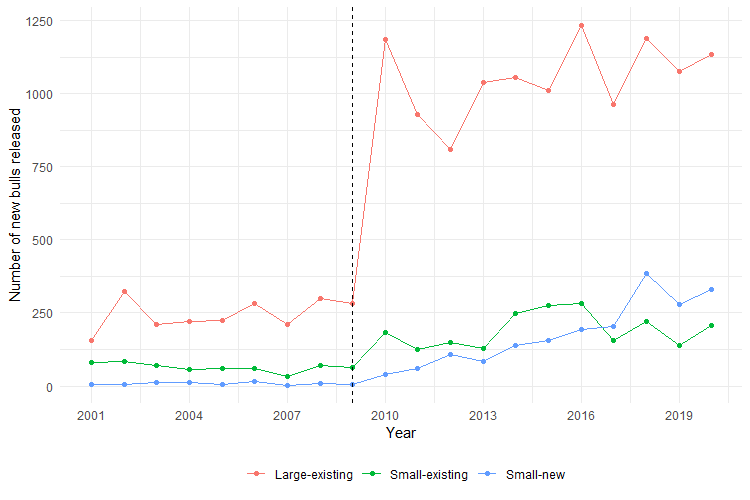
\includegraphics[width=16cm]{figures/new_bulls.png}
    \caption{Number of genotyped bulls by firm size\\ \small \textbf{Source}: NAAB}
    \label{fig:new_bulls} 
\end{figure}

\section{Empirical Approach}

\begin{figure}[H]
    \centering
    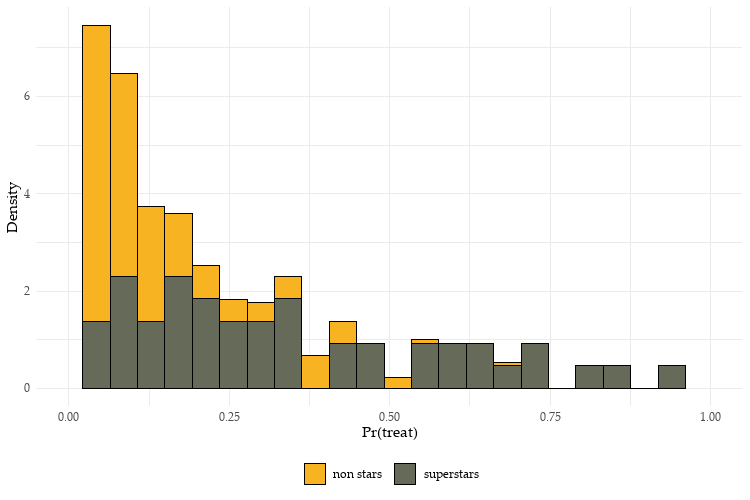
\includegraphics[width=16cm]{figures/common_support.png}
    \caption{Propensity score by class of bull}
    \label{fig:common_support} 
\end{figure}
\section{Results}
\begin{figure}[H]
    \centering
    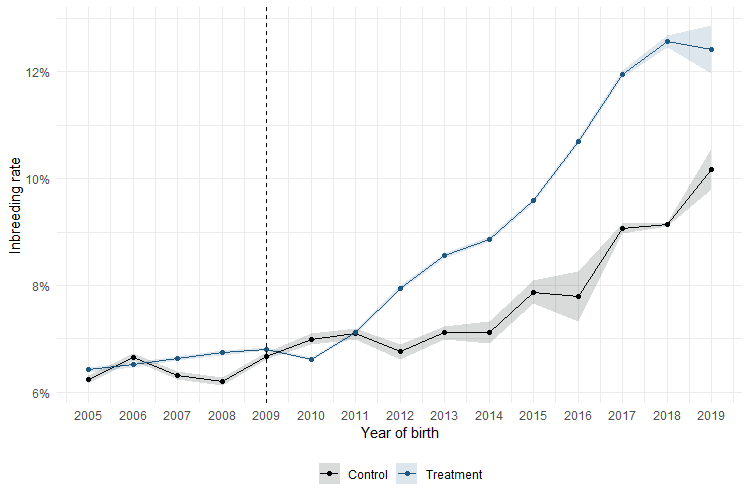
\includegraphics[width=14cm]{figures/inb_match.png}
    \caption{Average inbreeding rates in treatment and control groups}
    \label{fig:inb_match} 
\end{figure}
\section{Conclusion}


\newpage
\bibliography{references}
\end{document}
